\section{Discrete Time Behavior} \label{sec:discrete_time_behavior}
So far, we've considered that the system is continuous time. 
This is a reasonable assumption, if we have a high sampling time $\Delta t$, compared to the dynamics, i.e., $\| \Delta t \, \dot{\vecs \xi} \| \ll 1$.
However, any digital controller sends a discrete control signal. To reject the disturbances in the presence of obstacles, a high control force is exerted (while remaining within the control robot's limits), hence $\| \Delta t \, \vecs \tau^c \| \gg 1$. 
In this case, it is crucial to analyze the discrete-time system to guarantee stability, as high damping can lead to unstable behavior, see Figure~\ref{fig:discrete_controller_parameters_comparison}).

\begin{figure}[htbp]
\centering
  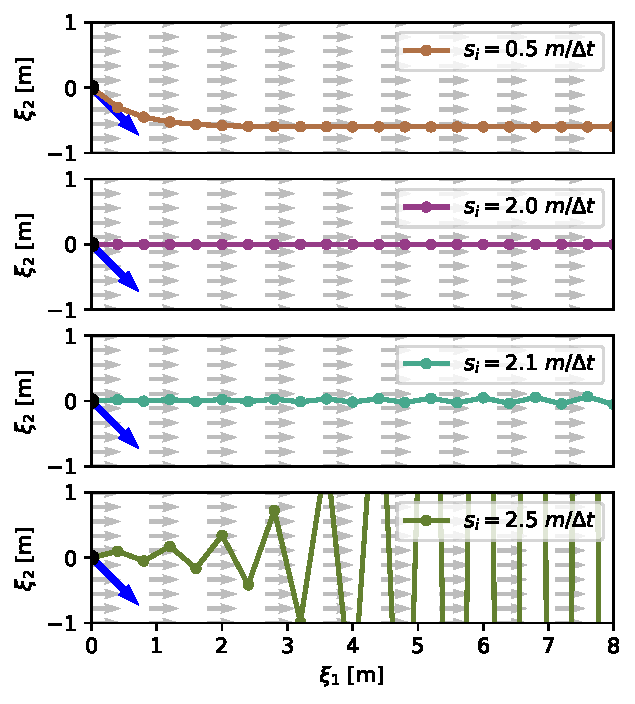
\includegraphics[width=\columnwidth]{figures/discrete_controller_parameters_comparison}
  \caption{A point-like agent with an initial velocity (blue arrow) of $\{ \dot{\vecs \xi} \}_0 = [1 \; -1]^T$ is guided by the desired velocity $\vect f(\vecs \xi) = [1, 0]^T$ (gray arrow), and a control matrix $\matd{D}$ with damping values $s_i$ equal in all directions, where $m = m^{\mathrm{min}}$ is the smallest eigenvalue of the inertia matrix. 
  Damping values above $s_i = 2.0 m / \Delta t$ lead to unstable behavior where the higher value leads to higher oscillations. Conversely, the lowest value leads to more deviation from the straight trajectory resulting from the higher impedance. The critical value of $s_i = 2.0 m / \Delta t$ results in stable behavior with immediate correction to the desired velocity.}
  \label{fig:discrete_controller_parameters_comparison}
\end{figure}

For the discrete-time system, the position and velocity of the agent evolve as follows:
\begin{equation}
	\begin{bmatrix}
	 \vecs \xi_{t+1} \\ \dot{\vecs \xi}_{t+1}
	\end{bmatrix}
	=
	\begin{bmatrix}
	 \vecs \xi_{t} \\ \dot{\vecs \xi}_{t}
	\end{bmatrix}
	+ 
	\Delta t 
	\begin{bmatrix}
		\dot{\vecs \xi}_{t} \\ \ddot{\vecs \xi}_t 
	\end{bmatrix}
	\label{eq:discrete_time_dynamics}
\end{equation}

\begin{lemma}
	Let us consider a discrete-time system with the state as given in Eq.~\eqref{eq:discrete_time_dynamics}, and is governed by the controller from Eq.~\eqref{eq:control_command} and damping matrix $\matd{D}$ defined in Eq.~\eqref{eq:damping_summation}.
	The system is BIBO (bounded-input, bounded-stable) with respect input the desired velocity $\vect f(\vecs \xi)$ the velocity, and as output the agent's velocity $\dot{\vecs \xi}$ such that $\lim_{t \rightarrow \infty} \| \dot{\vect \xi} \| < \infty$, if all damping values are limited as $s_{i} \leq 2 \min \left( \text{eig}\left(\matd{M}\right)  \right) / \Delta t$.
\end{lemma}

\begin{proof}
The evolution of the discrete-time feedback system is given as:
\begin{equation}
	\begin{split}
	& \begin{bmatrix}
	 \vecs \xi_{t+1} \\ \dot{\vecs \xi}_{t+1}
	\end{bmatrix}
	=
	\begin{bmatrix}
		\vect \xi_t + \Delta t  \; \dot{\vect \xi}_t \\ \
		\dot{\vecs \xi}_t + \Delta t \, \matd{M}^{-1} \left( \matd{D} \left( \vect f(\vecs \xi_t) - \dot{\vecs \xi}_t \right) - \matr C \right)
	\end{bmatrix} \\
	&  = %\approx
	\begin{bmatrix}
		\matr{I} & \matr{I} \Delta t \\
		\vect{0} & \matr{I} - \Delta t \matd{M}^{-1} \matd D 
	\end{bmatrix}
	\begin{bmatrix}
		\vect \xi_t \\ \dot{\vect \xi}_t
	\end{bmatrix}
	+ \begin{bmatrix}
		\vect{0} \\ 
		\Delta t \, \matd{M}^{-1} \matd{D} 
	\end{bmatrix}
	\hat{\vect f}(\vecs \xi_t) 
	% & \approx 
	% \begin{bmatrix}
	% 	1 & \Delta t \\
	% 	\Delta t \matd{M}^{-1} \matd D \frac{\partial \vect f}{\partial \vecs \xi} & 1 - \Delta t \matd{M}^{-1} \matd D 
	% \end{bmatrix}
	% \begin{bmatrix}
	% 	\vect \xi_t \\ \dot{\vect \xi}_t
	% \end{bmatrix}
	\label{eq:discrete_time_proof}
	\end{split}
\end{equation}
where $\hat{\vect f}(\vecs \xi_t) = \vect f(\vecs \xi_t) - \matd{D}^{-1} C$.  The dependency on the state $\vecs \xi$ of the matrices $\matd{M}$, $\matd{D}$, and $\matd{C}$ are omitted for brevity. $\matr{I} \in \mathbb{R}^{N \times N}$ denotes the identity matrix.
As we look at global stability, we look at the updated velocity $\hat{\vect f}(\vecs \xi_t) = \vect f(\vecs \xi_t) - \matd{D}^{-1} \matd{C}$. Since the Coriolis force is bounded, it follows that if the system is BIBO stable for $\hat{\vect f}(\vect \xi_t)$, then it is also BIBO stable for $\vect f(\vecs \xi_t)$ 

BIBO stability of a discrete-time system requires that all the eigenvalues of the feedback matrix are smaller or equal to one \cite{friedland2012control}.
The eigenvalues of the above feedback system are given as:
\begin{equation}
	\vect \lambda_1 = \text{eig}(\matr{I}) \qquad \vect \lambda_2 = \text{eig} \left(\matr{I} - \Delta t \, \matd{M}^{-1} \matd{D} \right)
\end{equation}
where both $\vect \lambda_1 \in \mathbb{R}^N$ and $\vect \lambda_2 \in \mathbb{R}^N$ denote a vector containing $N$ eigenvalues.
All eigenvalues of $\vect \lambda_{1, i} = 1, \; i = 1...N$, and enable a stable system. 
The second set of eigenvalues $\vect \lambda_2$  depends on the passive control term. 
However, since $\matd{M}$ and $\matd{D}$ are both positive definite, the eigenvalues are positive:
\begin{equation}
	\matd{M} > 0 \; , \;\; \matd{D} > 0 
	\qquad \Rightarrow \qquad
	\vect \lambda_{2, i} > 0 \quad i = 1...N
\end{equation}
% Furthermore, the system is stable if all eigenvalues are smaller or equal to one \cite{friedland2012control}. 
Hence, we only have to consider the upper limit, and the system is stable if the maximum eigenvalue is limited to:
\begin{equation}
	\max \left(\vect \lambda_2 \right) \leq 1 
	\quad \Rightarrow \quad
	s_{i} \leq 2 \min \Bigl( \text{eig}\bigl(\matd{M}\bigr)  \Bigr) / \Delta t
\end{equation}
\end{proof}

The stability guarantees provide BIBO stability, hence the boundedness of the output. 
Since the first eigenvalues equal one, there is no global asymptotic convergence. 
In fact, in the system from \eqref{eq:discrete_time_proof}, it can be observed that when the input dynamics are zero, i.e., $\vect f(\vecs \xi) = \vect 0$, the system immediately stops. But there is no convergence to a specific position.
However, in most cases, the desired system should only reach zero at the attractor position, and hence, we expect convergence to such a point.

Yet, asymptotic stability is not guaranteed for general nonlinear input dynamics. Especially for dynamics with high curvature and low damping value, the final trajectory can end up in limit cycles ((Figure~\ref{fig:discrete_controller_parameters_comparison_stable}).

\begin{figure}[htbp]
\centering
  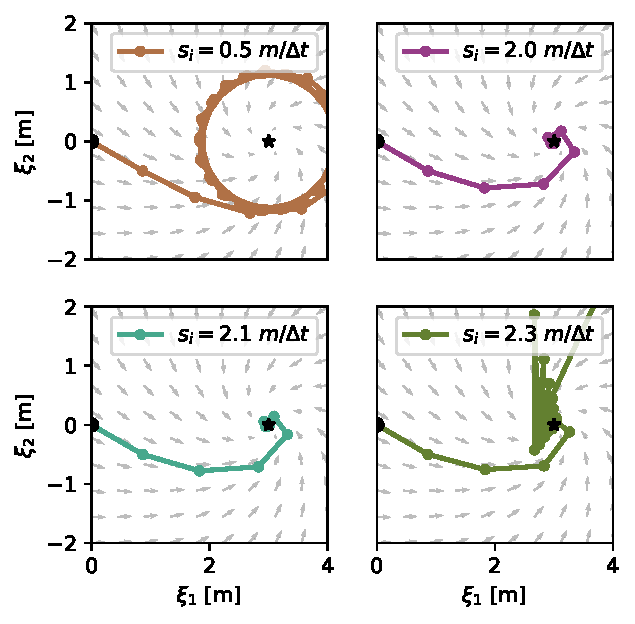
\includegraphics[width=\columnwidth]{figures/discrete_controller_parameters_comparison_stable}
\caption{A point-like agent which is following the desired dynamics of
$\vect f(\vecs \xi) = \matr R(\pi / 6) (\vect \xi  - \vect \xi^a)$ where $\matr R(\cdot) \in \mathbb{R}^{N \times N}$ is the rotation matrix, and $m$ is the mass of the agent. We assume equal damping values $s_i$.
The controller with a critical stiffness of $2.0 m / \Delta t$ leads to fast convergence and a stable system. With lower damping (top left), there is a large drift of the system, which converges to a limit cycle. 
The high damping of $2.3 m / \Delta t$ leads to an unstable system. 
Interestingly, with damping of $2.1 m / \Delta t$ in combination with the nonlinear dynamics, we obtain a visibly stable system.}
  \label{fig:discrete_controller_parameters_comparison_stable}
\end{figure}

% For a general nonlinear system no asymptotic convergence evaluation can be made. This is due to the fact, that for any system there is a slight drift due to the damping values.
% And hence, if there are high nonlinearities in the system it could happen that even with a stable system, the dynamics get caught in a limit cycle. However, for most common globally asymptotic systems (for velocity-position), the force controller as proposed leads to globally asymptotically stable behavior, too (Figure~\ref{fig:discrete_controller_parameters_comparison_stable}).

% \subsection{Intertial Drift}
% Let us assume that have strong damping in the direction of the obstacle, i.e., $s^{\mathrm{obs}} / m_i \gg 1$, where $m_i$ with $i = 1, .., N$ represent the eigenvalues of the mass matrix $\matd{M}$. 
% 
